\documentclass{article}
\usepackage[utf8]{inputenc}
\usepackage{url}
\usepackage{graphicx}
\usepackage{float}
\usepackage{indentfirst}
\usepackage{wrapfig}

\title{Auto Scrolling Platformer in Swift}
\author{Annika McCain, Caleb Stamper, Chazz Chandler, Jim Crowell \\ \small annikamccain@u.boisestate.edu, calebstamper@u.boisestate.edu,  \\ \small chazzchandler@u.boisestate.edu, jimcrowell@u.boisestate.edu} 

\date{October 2021}

\begin{document}

\maketitle

\section{Introduction}
The proposal is straight forward, especially if you consider the general use of Swift. We are going to design a platforming game in vain of Flappy Bird. Being that we have never coded in Swift or used the language before (indeed, that is the point of this assignment), we are not setting the bar overly high. We plan on dividing the code between us as evenly as possible and allowing people who have a preference for or are more skilled at certain segments than others to select a particular area they feel they might be more suited for. \hfill \break

There are several designs we have already sketched out and will implement as soon as coding begins. However, we also have goals set for additional features to improve the game, should we manage to get ahead of schedule or learn the code faster than we currently expect. \hfill \break 

The desire to use Swift is different for every member of the group, some had no other choices left, while others have been using Apple products and finally had an excuse to try Swift. In the following paragraphs you'll learn about the full design concepts we plan to implement as well as how we plan to design the code and when we would like to generate and work on specific sections of the code and design.\hfill \break

\section{Project Description}
\subsection{Platformer Design}
 The design is going to be kept more on the simple end of the spectrum, in order to reduce the overall complexity of the assignment and ensure the success of the group. The decision to make our project a game creation came about rather quickly, after which it we merely had to pick a genre. We finally settled on a platformer following the design similarities of Flappy Bird\cite{Flappybird}. Such a design would allow us to focus on the world design and art without having to worry as much about the many other possible moving parts of other more complex platforming games. Our philosophy was "fewer moving parts, fewer chances for failure," which is an old engineering standard. \hfill \break 

The primary concept of the game is to be a stationary player character in the X axis that can maneuver vertically on the Y Axis to navigate the platforms. This will be done by allowing the player character to jump with a tap input. Our first focus will be on having platforms generate at consistent intervals at identical heights, then slowly begin altering the heights that the platforms generate at, so as increase the difficulty as game time progresses.\hfill \break 

\subsection{General Game Info}
The game will include a standard heads-up display, which is intended to contain info such as how long the game has been played, the level the player is on and a high score. The menu will also include the ability to mute any audio we include and a suspend feature (think modern handhelds) so the user can take a break without losing their place. \hfill \break

The game level/difficulty will increment after either a certain number of platforms have passed or after a set amount of time has elapsed. As levels progress the speed at which platforms generate will increase to increase the difficulty. The level design has yet to be fully decided upon, there are many possible ways we have considered. Current favored idea is an auto-scroller, the general color palette of which will change upon succeeding an individual level. \hfill \break
    \begin{wrapfigure}{R}{0.3\textwidth}
        \centering
        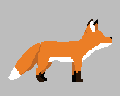
\includegraphics[width=0.25\textwidth]{fox.png}
        \caption{Game Sprite}
    \end{wrapfigure}
    
We also have settled on an overall game art style to be based off of a 16 bit, old-school style. This will allow for a simpler design while still inspiring a bit of nostalgic charm in the user (or at least, such is our hope). On the subject of art, the aesthetic is, as yet, undecided. Potential abounds, with everything from the "Green Hill Zone" feel of old platformers like Mario World or Sonic 2, to something with a bit more of a modern streak. Currently we have made a sprite (see Figure 1) but we have yet to decide if we want to go down this specific route. \hfill \break


\subsection{Additional Concepts}
The following items are dependant entirely upon how much the team is able to complete in the allotted time. One might think of them as "stretch goals", in the modern parlance. We initially set our goals very high as most designers do, and we slowly scaled things back to more feasible levels. We've moved our more lofty bells and whistles to a "maybe" pile, but we'd love to include them for not only quality of life but also overall polish. \hfill \break

A key addition we'd love to include is some possible series of collectibles for the user to strive to get while still having to maintain the pace of the platforms. Additionally, a possible power up to allow the user to double jump or jump higher than they typically do to improve platform traversal and provide more variety in terms of game feel for the user (this is the sort of philosophy espoused by Search Action/Metroidvania games). Regarding polish as a design concept, if all goes well, our artist may be able to implement biomes or other aesthetic/setting shifts as the game progresses.\hfill \break
\section{Evaluation}
Sense we will be designing a game will we need to test many cases that can go wrong. One round of testing will test if all the individual cases of failure (running into a wall, missing a platform, etc) work and will 'kill' the player. We will also need to ensure that our scoring system will be accurate with the amount of platforms that we have jumped on are correct. We might be able recruit some testers to see if they find any bugs with jumping distance, power ups, or placement of the generated platforms.
\section{Management}
\subsection{Timeline}
    \begin{figure}[H]
        \centering
        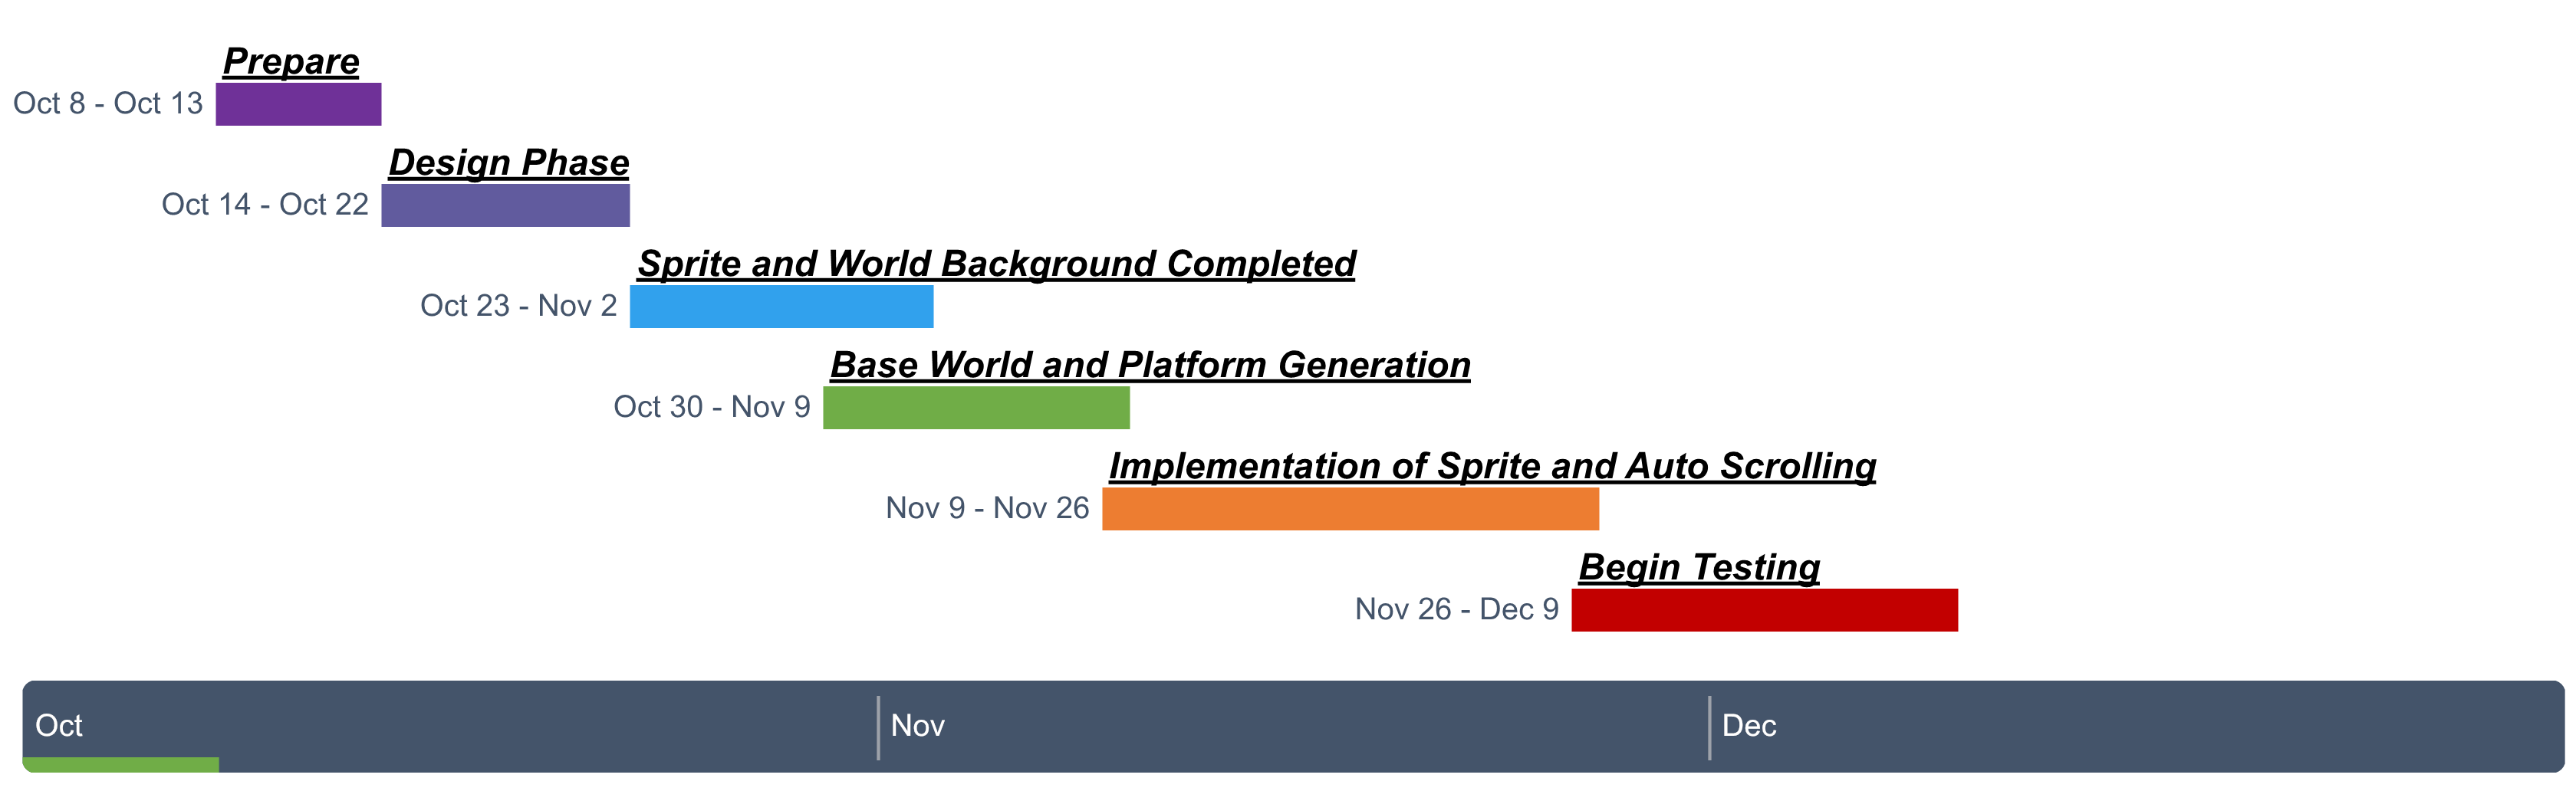
\includegraphics[width=1.25\columnwidth]{Project Outline.png}
        \caption{Timeline Gantt Chart}
    \end{figure}
\noindent Prepare (October 8 - 13) - installing Xcode and other dependencies on all group members machines
\\Design Phase (October 14 - 22) - brainstorming design of the world, items, additional sprites and creating sketches.
\\Sprite and World Background Completed (October 23 - November 2) - design completion.
\\Base World and Platform Generation (October 30 - November 9) - starting the base commands and setting up the game
\\Implementation of Sprite and Auto Scrolling (November 9 - 26) complete platform generation and begin user control of the sprite and adding the auto scrolling
\\ Begin Testing (November 26 - December 9) - The game should be playable and goes into testing
\subsection{Communication}
Currently, we have decided that our main point of contact is to use Discord. It is possible that in the future we might change it to text to make it easier to communicate everyone.
\subsection{Deviation of the Work}
At the moment we are uncertain as how we are going to split up who codes what but what we have decided is that we will brainstorm together to create the idea of the scenery and background and Annika will create them into digital pieces. We will reestablish who will code what when we get to that phases but for the time being we will share the burden to create the basic game controls.

\newpage

\bibliographystyle{plainnat}
\bibliography{refs}

\end{document}
